\documentclass[aspectratio=169]{beamer}

% VSE_FMV Presentation Template
\usetheme{Madrid}
\usecolortheme{default}

% Packages
\usepackage[utf8]{inputenc}
\usepackage[T1]{fontenc}
\usepackage{graphicx}
\usepackage{amsmath}
\usepackage{amsfonts}
\usepackage{amssymb}
\usepackage{tikz}
\usepackage{hyperref}

% Color scheme (VSE_FMV style - blue and gold)
\definecolor{vseblue}{RGB}{0,51,102}
\definecolor{vsegold}{RGB}{218,165,32}
\definecolor{lightgray}{RGB}{245,245,245}

\setbeamercolor{structure}{fg=vseblue}
\setbeamercolor{palette primary}{bg=vseblue,fg=white}
\setbeamercolor{palette secondary}{bg=vsegold,fg=white}
\setbeamercolor{palette tertiary}{bg=vseblue,fg=white}
\setbeamercolor{palette quaternary}{bg=vsegold,fg=white}
\setbeamercolor{titlelike}{parent=palette primary}
\setbeamercolor{block title}{bg=vseblue,fg=white}
\setbeamercolor{block body}{bg=lightgray,fg=black}

% Remove navigation symbols
\setbeamertemplate{navigation symbols}{}

% Footline with university name
\setbeamertemplate{footline}{
  \leavevmode%
  \hbox{%
  \begin{beamercolorbox}[wd=.333333\paperwidth,ht=2.25ex,dp=1ex,center]{author in head/foot}%
    \usebeamerfont{author in head/foot}\insertshortauthor
  \end{beamercolorbox}%
  \begin{beamercolorbox}[wd=.333333\paperwidth,ht=2.25ex,dp=1ex,center]{title in head/foot}%
    \usebeamerfont{title in head/foot}\insertshorttitle
  \end{beamercolorbox}%
  \begin{beamercolorbox}[wd=.333333\paperwidth,ht=2.25ex,dp=1ex,right]{date in head/foot}%
    \usebeamerfont{date in head/foot}\insertshortdate{}\hspace*{2em}
    \insertframenumber{} / \inserttotalframenumber\hspace*{2ex} 
  \end{beamercolorbox}}%
  \vskip0pt%
}

% Title page information
\title[Machine Learning in Finance]{Application of Machine Learning in Financial Markets}
\subtitle{An Overview of Predictive Analytics}
\author[Sarthak]{Sarthak}
\institute[JSPM University]{
  JSPM University\\
  Department of Finance and Management\\
  \vspace{0.3cm}
  \includegraphics[height=1.5cm]{jspm_logo.png} % Add your logo file
}
\date{\today}

\begin{document}

% Title slide
\begin{frame}
  \titlepage
\end{frame}

% Table of Contents
\begin{frame}{Outline}
  \tableofcontents
\end{frame}

% Section 1
\section{Introduction}

\begin{frame}{Introduction}
  \begin{block}{Overview}
    Machine Learning (ML) has revolutionized the financial industry by enabling:
    \begin{itemize}
      \item Automated trading systems
      \item Risk assessment and management
      \item Fraud detection
      \item Customer behavior prediction
    \end{itemize}
  \end{block}
  
  \vspace{0.5cm}
  
  \begin{alertblock}{Research Question}
    How can machine learning algorithms improve financial decision-making and risk management?
  \end{alertblock}
\end{frame}

% Section 2
\section{Literature Review}

\begin{frame}{Literature Review}
  \begin{columns}[T]
    \begin{column}{0.5\textwidth}
      \textbf{Key Studies:}
      \begin{itemize}
        \item Neural Networks in Trading (2020)
        \item Deep Learning for Risk Analysis (2021)
        \item AI-Driven Portfolio Management (2022)
      \end{itemize}
    \end{column}
    
    \begin{column}{0.5\textwidth}
      \textbf{Research Gaps:}
      \begin{itemize}
        \item Limited real-time implementation
        \item Interpretability challenges
        \item Regulatory concerns
      \end{itemize}
    \end{column}
  \end{columns}
\end{frame}

% Section 3
\section{Methodology}

\begin{frame}{Methodology}
  \begin{block}{Data Collection}
    \begin{itemize}
      \item Historical stock price data (2015-2024)
      \item Financial statements and ratios
      \item Market sentiment indicators
    \end{itemize}
  \end{block}
  
  \begin{block}{ML Algorithms Applied}
    \begin{enumerate}
      \item Random Forest Classifier
      \item Long Short-Term Memory (LSTM) Networks
      \item Support Vector Machines (SVM)
      \item Gradient Boosting Machines
    \end{enumerate}
  \end{block}
\end{frame}

\begin{frame}{Research Framework}
  \begin{center}
    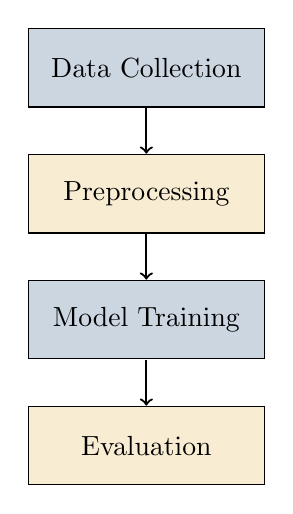
\begin{tikzpicture}[scale=0.8]
      % Data Collection
      \node[draw, rectangle, fill=vseblue!20, minimum width=3cm, minimum height=1cm] (data) at (0,0) {Data Collection};
      
      % Preprocessing
      \node[draw, rectangle, fill=vsegold!20, minimum width=3cm, minimum height=1cm] (prep) at (0,-2) {Preprocessing};
      
      % Model Training
      \node[draw, rectangle, fill=vseblue!20, minimum width=3cm, minimum height=1cm] (train) at (0,-4) {Model Training};
      
      % Evaluation
      \node[draw, rectangle, fill=vsegold!20, minimum width=3cm, minimum height=1cm] (eval) at (0,-6) {Evaluation};
      
      % Arrows
      \draw[->, thick] (data) -- (prep);
      \draw[->, thick] (prep) -- (train);
      \draw[->, thick] (train) -- (eval);
    \end{tikzpicture}
  \end{center}
\end{frame}

% Section 4
\section{Results}

\begin{frame}{Results}
  \begin{table}
    \centering
    \caption{Model Performance Comparison}
    \begin{tabular}{|l|c|c|c|}
      \hline
      \textbf{Algorithm} & \textbf{Accuracy} & \textbf{Precision} & \textbf{Recall} \\
      \hline
      Random Forest & 87.3\% & 85.6\% & 88.9\% \\
      \hline
      LSTM & 89.5\% & 88.2\% & 90.1\% \\
      \hline
      SVM & 84.7\% & 83.1\% & 85.5\% \\
      \hline
      Gradient Boosting & 88.9\% & 87.4\% & 89.6\% \\
      \hline
    \end{tabular}
  \end{table}
  
  \vspace{0.5cm}
  
  \begin{itemize}
    \item LSTM networks showed the highest accuracy
    \item All models exceeded 80\% accuracy threshold
    \item Ensemble methods improved prediction stability
  \end{itemize}
\end{frame}

% Section 5
\section{Discussion}

\begin{frame}{Key Findings}
  \begin{block}{Advantages}
    \begin{itemize}
      \item Superior prediction accuracy compared to traditional methods
      \item Ability to process large-scale data in real-time
      \item Adaptive learning from market changes
    \end{itemize}
  \end{block}
  
  \begin{alertblock}{Challenges}
    \begin{itemize}
      \item Black-box nature of deep learning models
      \item Overfitting risks with limited data
      \item Computational resource requirements
    \end{itemize}
  \end{alertblock}
\end{frame}

\begin{frame}{Practical Implications}
  \begin{enumerate}
    \item \textbf{For Financial Institutions:}
    \begin{itemize}
      \item Enhanced risk management capabilities
      \item Improved customer segmentation
    \end{itemize}
    
    \vspace{0.3cm}
    
    \item \textbf{For Investors:}
    \begin{itemize}
      \item Data-driven investment strategies
      \item Better portfolio diversification
    \end{itemize}
    
    \vspace{0.3cm}
    
    \item \textbf{For Regulators:}
    \begin{itemize}
      \item Need for AI governance frameworks
      \item Transparency requirements
    \end{itemize}
  \end{enumerate}
\end{frame}

% Section 6
\section{Conclusion}

\begin{frame}{Conclusion}
  \begin{block}{Summary}
    \begin{itemize}
      \item Machine learning significantly enhances financial decision-making
      \item LSTM networks demonstrate superior performance in time-series prediction
      \item Integration with traditional analysis methods yields best results
    \end{itemize}
  \end{block}
  
  \vspace{0.5cm}
  
  \begin{block}{Future Research Directions}
    \begin{itemize}
      \item Explainable AI (XAI) in financial applications
      \item Integration of alternative data sources
      \item Real-time adaptive learning systems
    \end{itemize}
  \end{block}
\end{frame}

% References
\begin{frame}{References}
  \begin{thebibliography}{99}
    \bibitem{ref1} Smith, J. (2022). \textit{Deep Learning in Finance}. Financial Analytics Press.
    
    \bibitem{ref2} Chen, L., \& Wang, M. (2021). Machine Learning for Stock Prediction. \textit{Journal of Financial Technology}, 15(3), 234-256.
    
    \bibitem{ref3} Anderson, K. (2023). AI and Risk Management in Banking. \textit{International Finance Review}, 28(2), 145-167.
    
    \bibitem{ref4} Patel, R., \& Kumar, S. (2022). Ensemble Methods in Financial Forecasting. \textit{Computational Finance}, 12(4), 78-95.
  \end{thebibliography}
\end{frame}

% Thank you slide
\begin{frame}[plain]
  \begin{center}
    \vspace{1.5cm}
    {\Huge \textcolor{vseblue}{\textbf{Thank You!}}}
    
    \vspace{1cm}
    
    {\Large Questions \& Discussion}
    
    \vspace{1.5cm}
    
    {\large Sarthak}\\
    \vspace{0.3cm}
    {\large JSPM University}\\
    \vspace{0.3cm}
    {\normalsize sarthak@jspm.edu.in}
  \end{center}
\end{frame}

\end{document}
